% !TEX root = ../../book_ML.tex

\chapter{Giải tích ma trận}

% for increase vertical distance in matrix
\def\largevspace{\renewcommand{\arraystretch}{2}}
\def\smallvspace{\renewcommand{\arraystretch}{1}}

% \index{giải tcismatrix calculus}
% \section{Đạo hàm của hàm nhiều biến }
% \textit{Trong chương này, chúng ta sẽ giả sử rằng các đạo hàm tồn tại. Chúng ta sẽ xét hai trường hợp: i) Hàm số nhận giá trị là ma trận (vector) và cho giá trị là một số thực vô hướng; và ii) Hàm số nhận giá trị là một số vô hướng hoặc vector và cho giá trị là một vector.
% }
\vspace{-1.2in}
Giả sử rằng các gradient tồn tại trong toàn bộ chương. Tài liệu tham khảo
chính của chương là \textit{Matrix calculus -- Stanford}
(\url{https://goo.gl/BjTPLr}).

\largevspace
\section{Gradient của hàm trả về một số vô hướng}
\index{gradient}
\index{gradient!gradient bậc nhất -- first-order gradient}
\index{gradient!first-order gradient -- gradient bậc nhất}
\index{partial derivative -- đạo hàm riêng}
\index{đạo hàm riêng -- partial derivative}
\textit{Gradient bậc nhất} ({first-order gradient}) hay viết gọn là
{gradient} của một hàm số $f(\bx): \mathbb{R}^n
\rightarrow
\mathbb{R}$
theo $\bx$, ký hiệu là $\nabla_{\bx} f(\bx)$, được định nghĩa bởi
\begin{equation}
\label{eqn:grvector1}
\nabla_{\bx} f(\bx) \triangleq
\left[
\begin{matrix}
\dfrac{\partial f(\bx)}{\partial x_1} \\\
\dfrac{\partial f(\bx)}{\partial x_2} \\\
\vdots \\\
\dfrac{\partial f(\bx)}{\partial x_n}
\end{matrix}
\right] \in \mathbb{R}^n,
\end{equation}
trong đó $\displaystyle\dfrac{\partial f(\bx)}{\partial x_i}$ là \textit{đạo hàm
riêng} của hàm số theo thành phần thứ $i$ của
vector $\bx$. Đạo hàm này được tính khi tất cả các biến, ngoài $x_i$, được giả sử
là hằng số. Nếu không có thêm biến nào khác, $\nabla_{\bx}f(\bx)$ thường được
viết gọn là $\nabla f(\bx)$. {Gradient của hàm số này là một vector có
cùng chiều với vector đang được lấy gradient}. Tức nếu vector được viết ở dạng
cột thì gradient cũng phải được viết ở dạng cột.% Ta cần tính đạo hàm riêng theo từng thành phần của vector rồi sắp xếp chúng lại theo đúng thứ tự ban đầu.

\index{gradient!gradient bậc hai -- second-order gradient}
\index{gradient!second-order gradient -- gradient bậc hai}
\index{Hesse -- Hessian}
\index{Hessian -- Hesse}
\textit{Gradient bậc hai} ({second-order gradient}) của hàm số trên còn
được gọi là \textit{Hesse} (Hessian) và được định nghĩa như sau:

\begin{equation}
\label{eqn:hessian1}
\nabla^2 f(\bx) \triangleq
\bmt
\dfrac{\partial^2 f(\bx)}{\partial x_1^2} & \dfrac{\partial^2 f(\bx)}{\partial x_1\partial x_2} & \dots & \dfrac{\partial^2 f(\bx)}{\partial x_1\partial x_n} \\\
\dfrac{\partial^2 f(\bx)}{\partial x_2\partial x_1} & \dfrac{\partial^2 f(\bx)}{\partial x_2^2} & \dots & \dfrac{\partial^2 f(\bx)}{\partial x_2\partial x_n} \\\
\vdots & \vdots & \ddots & \vdots \\\
\dfrac{\partial^2 f(\bx)}{\partial x_n\partial x_1} & \dfrac{\partial^2 f(\bx)}{\partial x_n\partial x_2} & \dots & \dfrac{\partial^2 f(\bx)}{\partial x_n^2}
\emt \in \mathbb{S}^{n}.
\end{equation}


Gradient của một hàm số $f(\bX): \mathbb{R}^{n \times m} \rightarrow
\mathbb{R}$ {theo ma trận} $\bX$ được định nghĩa là
\begin{equation}
\label{eqn:grmatrix1}
\nabla f(\bX) =
\bmt
\dfrac{\partial f(\bX)}{\partial x_{11}} & \dfrac{\partial f(\bX)}{\partial x_{12}} & \dots & \dfrac{\partial f(\bX)}{\partial x_{1m}} \\\
\dfrac{\partial f(\bX)}{\partial x_{21}} & \dfrac{\partial f(\bX)}{\partial x_{22}} & \dots & \dfrac{\partial f(\bX)}{\partial x_{2m}} \\\
\vdots & \vdots & \ddots & \vdots \\\
\dfrac{\partial f(\bX)}{\partial x_{n1}} & \dfrac{\partial f(\bX)}{\partial x_{n2}} & \dots & \dfrac{\partial f(\bX)}{\partial x_{nm}}
\emt \in \mathbb{R}^{n \times m}.
\end{equation}
\newnote{}{
Gradient của hàm số $f: \R^{m\times n} \rightarrow \R$ là một ma trận trong
$\R^{m\times n}.$
}
Cụ thể, để tính gradient của một hàm $f: \R^{m\times n} \rightarrow \R$, ta tính
đạo hàm riêng của hàm số đó theo từng thành
phần của ma trận {khi toàn bộ các thành phần khác được giả sử là hằng
số}. Tiếp theo, ta sắp xếp các đạo hàm riêng tính được theo đúng thứ tự
trong ma trận.

{\textit{Ví dụ}}: Xét hàm số $f: \mathbb{R}^2 \rightarrow \mathbb{R}$, $f(\bx) =
x_1 ^2 + 2x_1x_2 + \sin(x_1) + 2$. Gradient bậc nhất theo $\bx$ của hàm số đó là
\begin{equation*}
\nabla f(\bx) =
\bmt
\dfrac{\partial f(\bx)}{\partial x_1} \\\
\dfrac{\partial f(\bx)}{\partial x_2}
\emt = \bmt
2x_1 + 2x_2 + \cos(x_1) \\\
2x_1
\emt.
\end{equation*}

Gradient bậc hai theo $\bx$, hay Hesse là
% \begin{equation*}
$$
\nabla^2 f(\bx) =
\bmt
\dfrac{\partial^2 f(\bx)}{\partial x_1^2} & \dfrac{\partial f^2(\bx)}{\partial x_1\partial x_2} \\\
\dfrac{\partial^2 f(\bx)}{\partial x_2\partial x_1} & \dfrac{\partial f^2(\bx)}{\partial x_2^2}
\emt =
\bmt
2 - \sin(x_1) & 2 \\\
2 & 0
\emt.$$
% \end{equation*}
Chú ý rằng {Hesse} luôn là một ma trận đối xứng.


\section{Gradient của hàm trả về vector }

\index{hàm trả về vector -- vector-valued function}
\index{vector-valued function -- hàm trả về vector}
Những hàm số mà đầu ra là một vector được gọi là \textit{hàm trả về vector} (vector-valued function).

Xét một hàm trả về vector với đầu vào là một số thực $v(x):
\mathbb{R} \rightarrow
\mathbb{R}^n $:
\smallvspace
\begin{equation}
\label{eqn:vectorvalued}
v(x) =
\bmt
v_1(x) \\\
v_2(x) \\\
\vdots \\\
v_n(x)
\emt.
\end{equation}
Gradient của hàm số này theo $x$ là một {vector hàng} như sau:
\begin{equation}
\label{eqn:grvectorvalued}
\nabla v(x) \triangleq
\bmt
\dfrac{\partial v_1(x)}{\partial x} & \dfrac{\partial v_2(x)}{\partial x} &
\dots & \dfrac{\partial v_n(x)}{\partial x}
\emt.
\end{equation}
Gradient bậc hai của hàm số này có dạng:
\begin{equation}
\label{eqn:hessianvectorvalued}
\nabla^2 v(x) \triangleq
\left[
\begin{matrix}
\dfrac{\partial^2 v_1(x)}{\partial x^2} & \dfrac{\partial^2 v_2(x)}{\partial x^2} & \dots & \dfrac{\partial^2 v_n(x)}{\partial x^2}
\end{matrix}
\right].
\end{equation}

\vd Cho một vector $\mathbf{a} \in \mathbb{R}^n$ và một hàm số trả về
vector $v(x) = x\mathbf{a}$, gradient và Hesse của nó lần lượt là
\begin{equation}
\nabla v(x) = \mathbf{a}^T, ~~~ \nabla^2 v(x) = \mathbf{0} \in \mathbb{R}^{1\times n}.
\end{equation}
Xét một hàm trả về vector với {đầu vào là một vector}
$h(\bx):\mathbb{R}^k \rightarrow \mathbb{R}^n$, gradient của nó là
\begin{eqnarray}
\label{eqn:gdvectorvector}
\nabla h(\bx) &\triangleq &
\bmt
\dfrac{\partial h_1(\bx)}{\partial x_1} & \dfrac{\partial h_2(\bx)}{\partial x_1} & \dots & \dfrac{\partial h_n(\bx)}{\partial x_1} \\\
\dfrac{\partial h_1(\bx)}{\partial x_2} & \dfrac{\partial h_2(\bx)}{\partial x_2} & \dots & \dfrac{\partial h_n(\bx)}{\partial x_2} \\\
\vdots & \vdots & \ddots & \vdots \\\
\dfrac{\partial h_1(\bx)}{\partial x_k} & \dfrac{\partial h_2(\bx)}{\partial x_k} & \dots & \dfrac{\partial h_n(\bx)}{\partial x_k}
\emt =
\bmt
\nabla h_1(\bx) & \dots & \nabla h_n(\bx)
\emt \in \mathbb{R}^{k\times n}.
\end{eqnarray}

\newnote{}{
Gradient của hàm số $g: \mathbb{R}^m \rightarrow \mathbb{R}^n$ là
một ma trận thuộc $\mathbb{R}^{m \times n}$.
}

Gradient bậc hai của hàm số trên là một {mảng ba chiều}. Trong phạm vi của cuốn
sách, chúng ta sẽ không xét gradient bậc hai của các hàm số $g: \mathbb{R}^m
\rightarrow \mathbb{R}^n$.




% Với các hàm số \textit{matrix-valued} nhận giá trị đầu vào là ma trận, tôi
% cũng xin không đề cập ở đây. Tuy nhiên, ở phần dưới, khi tính toán đạo hàm cho
% các hàm cho giá trị là số thực, chúng ta vẫn có thể sẽ sử dụng khái niệm này.

Trước khi đến phần tính gradient của các hàm số thường gặp, chúng ta cần biết hai
tính chất quan trọng khá giống với gradient của hàm một biến.


\section{Tính chất quan trọng của gradient}
\index{quy tắc tích -- product rule}
\index{product rule -- quy tắc tích}
\subsection{Quy tắc tích}

Giả sử các biến đầu vào là một ma trận và các hàm số có chiều phù hợp để phép
nhân ma trận thực hiện được. Ta có
\begin{equation}
\label{eqn:productrules}
\nabla\left( f(\bX)^Tg(\bX) \right) = \left(\nabla f(\bX)\right) g(\bX) +
\left(\nabla g(\bX)\right) f(\bX).
\end{equation}
Quy tắc này tương tự như quy tắc tính đạo hàm của tích các hàm $f, g: \R \rightarrow \R$:
\begin{equation*}
\left(f(x)g(x)\right)' = f'(x)g(x) + g'(x)f(x).
\end{equation*}
Lưu ý rằng tính chất giao hoán không còn đúng với vector và ma trận, vì vậy nhìn chung
\begin{equation}
\nabla\left( f(\bX)^Tg(\bX) \right) \neq  g(\bX)\left(\nabla f(\bX)\right) +
f(\bX)\left(\nabla g(\bX)\right).
\end{equation}
Biểu thức bên phải có thể không xác định khi chiều của các ma trận lệch nhau.

\index{quy tắc chuỗi -- chain rule}
\index{chain rule -- quy tắc chuỗi}
\subsection{Quy tắc chuỗi}

Quy tắc chuỗi được áp dụng khi tính gradient của các hàm hợp:
\begin{equation}
\label{eqn:chainrules}
\nabla_{\bX} g(f(\bX)) = (\nabla_{\bX} f) (\nabla_{f}g).
\end{equation}

Quy tắc này cũng giống với quy tắc trong hàm một biến:
\begin{equation*}
(g(f(x)))' = f'(x)g'(f).
\end{equation*}
Một lưu ý nhỏ nhưng quan trọng khi làm việc với tích các ma trận là sự phù hợp
về kích thước của các ma trận trong tích.
\section{Gradient của các hàm số thường gặp }

\subsection{$f(\bx) = \mathbf{a}^T\bx$}

Giả sử $\mathbf{a}, \bx \in \mathbb{R}^n$, ta viết lại $f(\bx) =
\mathbf{a}^T\bx = a_1 x_1 + a_2 x_2 + \dots + a_nx_n$.
% f(\bx) = \mathbf{a}^T\bx = a_1 x_1 + a_2 x_2 + \dots + a_nx_n
% \end{equation*}

Nhận thấy $\dfrac{\partial f(\bx)}{\partial x_i} = a_i, ~
\forall i = 1, 2\dots, n$.
% \begin{equation*}
% \dfrac{\partial f(\bx)}{\partial x_i} = a_i, ~ \forall i = 1, 2\dots, n
% \end{equation*}

\smallvspace
Vậy, $\nabla_{\bx} (\ba^T\bx) = \bmt a_1 & a_2 & \dots & a_n \emt^T = \ba$.

Ngoài ra, vì $\mathbf{a}^T\bx = \bx^T\mathbf{a}$ nên $\nabla_{\bx} (\bx^T\mathbf{a}) =
\mathbf{a}$.
% \begin{equation*}
% \nabla (\bx^T\mathbf{a}) = \mathbf{a}
% \end{equation*}


\subsection{$f(\bx) = \mathbf{Ax}$}
Đây là một hàm trả về vector $f: \mathbb{R}^n \rightarrow \mathbb{R}^{m} $ với
$\bx \in \mathbb{R}^n, \mathbf{A} \in \mathbb{R}^{m\times n}$. Giả sử
$\mathbf{a}_i$ là {hàng} thứ $i$ của ma trận $\mathbf{A}$. Ta có
\begin{equation*}
\mathbf{Ax}  =
\bmt
\mathbf{a}_1\bx \\\
\mathbf{a}_2\bx \\\
\vdots\\\
\mathbf{a}_m\bx
\emt.
\end{equation*}
Từ định nghĩa \eqref{eqn:gdvectorvector} và công thức gradient của $\ba_i\bx$,
có thể suy ra
\begin{equation}
\label{eqn:gdAx}
\nabla_{\bx} (\mathbf{Ax}) =
\bmt
\mathbf{a}_1^T & \mathbf{a}_2^T & \dots & \mathbf{a}_m^T
\emt = \mathbf{A}^T
\end{equation}
Từ đây suy ra đạo hàm của hàm số $f(\bx) = \bx = \mathbf{Ix}$ là
\begin{equation*}
\nabla \bx = \mathbf{I}
\end{equation*}
với
$\mathbf{I}$ là ma trận đơn vị.

\subsection{$f(\bx) = \bx^T\mathbf{A} \bx$}
Với $\bx \in \mathbb{R}^n, \mathbf{A} \in \mathbb{R}^{n\times n}$, áp dụng quy
tắc tích~\eqref{eqn:productrules} ta có
\begin{eqnarray}
\nonumber
\nabla f(\bx) &=& \nabla \left(\left(\bx^T\right) \left(\mathbf{Ax}\right)\right) \\\
\nonumber
&=& \left(\nabla (\bx)\right) \mathbf{Ax} + \left(\nabla (\mathbf{Ax})\right)\bx \\\
\nonumber
& = & \mathbf{IAx} + \mathbf{A}^T\bx \\\
\label{eqn:gdxTAx}
& = & (\mathbf{A} + \mathbf{A}^T)\bx.
\end{eqnarray}
Từ \eqref{eqn:gdxTAx} và \eqref{eqn:gdAx}, có thể suy ra
\begin{math}
\nabla^2 \bx^T\mathbf{Ax} = \mathbf{A}^T + \mathbf{A}.
\end{math}
Nếu $\mathbf{A}$ là một ma trận đối xứng, ta có
$
\nabla \bx^T\mathbf{A}\bx = 2\mathbf{Ax},
\nabla^2 \bx^T\mathbf{Ax} = 2\mathbf{A}.
$

Nếu $\mathbf{A}$ là ma trận đơn vị, tức $f(\bx) = \bx^T\mathbf{Ix} = \bx^T\bx = \|\bx\|_2^2$, ta có
\begin{equation}
\nabla \|\bx\|_2^2 = 2\bx,~~~
\nabla^2 \|\bx\|_2^2 = 2\mathbf{I}.
\end{equation}


\subsection{$f(\bx) = \|\mathbf{Ax} - \mathbf{b}\|_2^2 $}
\label{sec:gr_squarenorm2}
Có hai cách tính gradient của hàm số này:
\begin{itemize}
\item {Cách 1:} Trước hết, khai triển:
\begin{eqnarray}
\nonumber
f(\bx) &=& \|\mathbf{Ax} - \mathbf{b}\|_2^2 = (\mathbf{Ax} - \mathbf{b})^T(\mathbf{Ax} - \mathbf{b}) = (\bx^T\mathbf{A}^T - \mathbf{b}^T) (\mathbf{Ax} - \mathbf{b}) \\\ \nonumber
&=& \bx^T\mathbf{A}^T\mathbf{Ax} - 2 \mathbf{b}^T\mathbf{Ax} + \mathbf{b}^T\mathbf{b}.
\end{eqnarray}
Lấy gradient cho từng số hạng rồi cộng lại ta có
\begin{equation*}
\nabla \|\mathbf{Ax} - \mathbf{b}\|_2^2 = 2\mathbf{A}^T\mathbf{A}\bx - 2\mathbf{A}^T\mathbf{b} = 2\mathbf{A}^T(\mathbf{Ax} - \mathbf{b}).
\end{equation*}

\item {Cách 2:} Sử dụng $\nabla (\mathbf{Ax} - \mathbf{b}) =
\mathbf{A}^T$ và $\nabla \|\bx\|_2^2 = 2\bx$ và quy tắc chuỗi~\eqref{eqn:chainrules}, ta cũng sẽ thu được kết quả tương tự.
\end{itemize}

\subsection{$f(\bx) = \mathbf{a}^T\bx\bx^T\mathbf{b}$}
Viết lại $f(\bx) = (\mathbf{a}^T\bx)(\bx^T\mathbf{b})$ và dùng
quy tắc tích~\eqref{eqn:productrules}, ta có
\begin{equation*}
\nabla (\mathbf{a}^T\bx\bx^T\mathbf{b}) = \mathbf{a} \bx^T\mathbf{b} +
\mathbf{b}\mathbf{a}^T\bx = \mathbf{ab}^T\bx + \mathbf{b}\mathbf{a}^T\bx=
(\mathbf{ab}^T + \mathbf{ba}^T)\bx,
\end{equation*}
ở đây ta đã sử dụng tính chất $\mathbf{y}^T\mathbf{z} = \mathbf{z}^T\mathbf{y}$.
% và tích của một số thực với một vector cũng bằng tích của vector và số thực đó.

\subsection{$f(\bX) = \trace(\bA\bX)$}
Giả sử $\bA \in \R^{n\times m}, \bX = \R^{m\times n}$, và $\bB = \bA\bX \in \R^
{n \times n}$. Theo định nghĩa của trace:
\begin{equation}
f(\bX) = \trace(\bA\bX) = \trace(\bB) = \sum_{j = 1}^n {b_{jj}} =
\sum_{j=1}^n\sum_{i=1}^n a_{ji}x_{ji}.
\end{equation}
Từ đó suy ra $\displaystyle\frac{\partial f(\bX)}{\partial x_{ij}} =
a_{ji}$. Theo định nghĩa~\eqref{eqn:grmatrix1}, ta có $\nabla_{\bX}\trace(\bA\bX) =
\bA^T$.

\subsection{$f(\bX) = \ba^T\bX\bb$}
Giả sử rằng $\ba \in \R^{m}, \bX \in R^{m\times n}, \bb \in \R^{n}$. Ta có
thể chứng minh được $$f(\bX) = \sum_{i=1}^m \sum_{j=1}^n x_{ij}a_ib_j.$$
Từ đó, sử dụng định nghĩa~\eqref{eqn:grmatrix1}, ta đạt được
\begin{equation}
\nabla_{\bX}(\ba^T\bX\bb^T) = \bmt
a_1b_1 &  a_1b_2 & \dots &a_1b_n \\
a_2b_1 &  a_2b_2 & \dots &a_2b_n \\
\dots & \dots & \ddots & \dots \\
a_mb_1 &  a_mb_2 & \dots &a_mb_n \\
\emt
= \ba\bb^T.
\end{equation}
% \begin{equation}

% \end{equation}

\subsection{$f(\bX) = \|\bX\|_F^2$}
% bằng cách viết lại $\|\bX\|_F^2 =
% \sum_{i=1}^n\sum_{j=1}^n x_{ij}^2$,
% ta có thể suy ra $\frac{\partial f}{\partial x_{ij}} = 2x_{ij}$. Từ đó,
% $\nabla \|\bX\|_F^2 = 2\bX$.
Giả sử $\bX \in \R^{n\times n}$, ta có
$$
\|\bX\|_F^2 =
\sum_{i=1}^n\sum_{j=1}^n x_{ij}^2 \Rightarrow \frac{\partial f}{\partial x_{ij}} = 2x_{ij} \Rightarrow \nabla \|\bX\|_F^2 = 2\bX.
$$


\subsection{$f(\bX) = \trace(\bX^T\bA\bX)$}
Giả sử rằng $\bX = \bmt \bx_1 & \bx_2 & \dots & \bx_n \emt \in \R^{m\times n},
\bA \in \R^{m\times m}$. Bằng cách khai triển
\begin{equation*}
\bX^T\bA\bX = \bmt \bx_1^T \\ \bx_2^T \\ \vdots \\ \bx_n^T \emt \bA \bmt
\bx_1 & \bx_2 & \dots, \bx_n \emt = \bmt
\bx_1^T\bA\bx_1 & \bx_1^T\bA\bx_2 & \dots & \bx_1^T\bA\bx_n \\
\bx_2^T\bA\bx_1 & \bx_2^T\bA\bx_2 & \dots & \bx_2^T\bA\bx_n \\
\dots & \dots & \ddots & \dots \\
\bx_n^T\bA\bx_1 & \bx_n^T\bA\bx_2 & \dots & \bx_n^T\bA\bx_n
\emt,
\end{equation*}
ta tính được $\trace(\bX^T\bA\bX) = \sum_{i=1}^n \bx_i^T\bA\bx_i$.

Sử dụng công thức $\nabla_{\bx_i}\bx_i^T\bA\bx_i = (\bA + \bA^T)\bx_i$, ta có
\begin{equation}
\nabla_{\bX} \trace(\bX^T\bA\bX) = (\bA + \bA^T) \bmt \bx_1 & \bx_2 & \dots &
\bx_n \emt = (\bA + \bA^T)\bX.
\end{equation}
Bằng cách thay $\bA = \bI$, ta cũng thu được $\nabla_{\bX}\trace(\bX^T\bX) =
\nabla_{\bX} \|\bX\|_F^2 = 2\bX$.

\subsection{$f(\bX) = \|\bA\bX - \bB\|_F^2$}
Bằng kỹ thuật hoàn toàn tương tự như đã làm trong Mục~\ref{sec:gr_squarenorm2},
ta thu được $$\nabla_{\bX} \|\bA\bX - \bB\|_F^2 = 2\bA^T(\bA\bX - \bB).$$


\section{Bảng các gradient thường gặp}

% \subsection{Cho vector }

Bảng~\ref{tab:commongr} bao gồm gradient của các hàm số thường gặp với biến là
vector hoặc ma trận.


%% *****************************************************************************
\begin{table}
\centering
\caption{Bảng các gradient cơ bản.}
\label{tab:commongr}
\setlength{\tabcolsep}{0.5em}
{\normalsize \def\arraystretch{1.25}
\begin{tabular}{|l|l||l|l|}
\hline
$f(\bx) $                         & $ \nabla f(\bx) $                                         & $f(\bX)$ & $\nabla_{\bX} f(\bX)$\\ \hline
\hline
$ \bx $ & $\bI$ & $\trace(\bX)$ &$ \bI$ \\ \hline
$\mathbf{a}^T \bx $               & $\mathbf{a}$                                              & $\trace(\bA^T\bX)$         & $\bA$ \\ \hline
$\bx^T\mathbf{Ax}$                & $(\mathbf{A} + \mathbf{A}^T) \bx$                         &  $\trace(\bX^T\bA\bX)$        & $(\bA + \bA^T) \bX$ \\ \hline
$\bx^T \bx = \|\bx\|_2^2 $        & $2\bx$                                                    &  $\trace(\bX^T\bX) = \|\bX\|_F^2$        & $2\bX$\\ \hline
$ \|\mathbf{Ax-b} \|_2^2 $        & $ 2\mathbf{A}^T (\mathbf{Ax - b})$                        &  $\|\bA\bX - \bB \|_F^2$        & $2\bA^T(\bA\bX - \bB)$ \\ \hline
$\mathbf{a}^T(\bx^T\mathbf{x})\mathbf{b} $   & $2\mathbf{a}^T\mathbf{bx} $                               &  $\ba^T\bX\bb$        & $\ba\bb^T$ \\ \hline
$\mathbf{a}^T\bx\bx^T\mathbf{b} $ & $ (\mathbf{a}\mathbf{b}^T + \mathbf{b}\mathbf{a}^T) \bx $ &  $\trace(\bA^T\bX\bB)$        & $\bA\bB^T$\\ \hline
\end{tabular}}
\end{table}
%% *****************************************************************************

\section{Kiểm tra gradient}
\label{sec:check_grad}
\index{gradient!gradient xấp xỉ -- numerical gradient}
\index{gradient!numerical gradient -- gradient xấp xỉ}

Việc tính gradient của hàm nhiều biến thông thường khá phức tạp và rất dễ mắc
lỗi. Trong thực nghiệm, có một cách để kiểm tra liệu gradient tính được có chính
xác không. Cách này dựa trên định nghĩa của đạo hàm cho hàm một biến.

\subsection{Xấp xỉ đạo hàm của hàm một biến}
\label{sub:xap_xi_dao_ham_cua_ham_mot_bien}
Xét cách tính đạo hàm của hàm một biến theo định nghĩa:
\begin{equation}
\label{eqn:grdef1}
f'(x) = \lim_{\varepsilon \rightarrow 0}\frac{f(x + \varepsilon) -
f(x)}{\varepsilon}.
\end{equation}
Trên máy tính, ta có thể chọn $\varepsilon$ rất nhỏ, ví dụ $10^{-6}$, rồi xấp xỉ đạo hàm này bởi
\begin{equation}
f'(x) \approx \lim_{\varepsilon \rightarrow 0}\frac{f(x + \varepsilon) -
f(x)}{\varepsilon}.
\end{equation}
Trên thực tế, công thức xấp xỉ đạo hàm hai phía thường được sử dụng:
\begin{equation}
\label{eqn:grdef2}
f'(x) \approx \frac{f(x + \varepsilon) - f(x - \varepsilon)}{2\varepsilon}.
\end{equation}
Cách tính này được gọi là \textit{numerical gradient}. Có hai cách giải thích việc tại sao cách tính như~\eqref{eqn:grdef2} được sử dụng rộng rãi hơn:

* \textit{Bằng giải tích}

Sử dụng khai triển Taylor với $\varepsilon$ rất nhỏ, ta có hai xấp xỉ sau:
\begin{eqnarray}
f(x + \varepsilon) &\approx& f(x) + f'(x)\varepsilon + \frac{f"(x)}{2}
\varepsilon^2 + \frac{f^{(3)}}{6}\varepsilon^3 + \dots \\
f(x - \varepsilon) &\approx& f(x) - f'(x)\varepsilon + \frac{f"(x)}{2}
\varepsilon^2 - \frac{f^{(3)}}{6}\varepsilon^3 + \dots
\end{eqnarray}
%
Từ đó ta có:
\begin{eqnarray}
\label{eqn:numgrdef1}
\frac{f(x + \varepsilon) - f(x)}{\varepsilon} &\approx& f'(x) +
\frac{f"(x)}{2}\varepsilon + \dots =  f'(x) + O(\varepsilon). \\
\label{eqn:numgrdef2}
\frac{f(x + \varepsilon) - f(x - \varepsilon)}{2\varepsilon} &\approx& f'(x) +
\frac{f^{(3)}(x)}{6}\varepsilon^2 + \dots =  f'(x) + O(\varepsilon^2).
\end{eqnarray}
trong đó $O()$ là {Big O notation}.

Từ đó, nếu xấp xỉ đạo hàm bằng công thức~\eqref{eqn:numgrdef1}, sai số sẽ là $O(\varepsilon)$. Trong khi đó, nếu xấp xỉ đạo hàm bằng công
thức~\eqref{eqn:numgrdef2}, sai số sẽ là
$O(\varepsilon^2)$. Khi $\varepsilon$ rất nhỏ, $O(\varepsilon^2) \ll
O(\varepsilon)$, tức cách đánh giá sử dụng công thức~\eqref{eqn:numgrdef2} có sai
số nhỏ hơn, và vì vậy nó được sử dụng phổ biến hơn.

% Chúng ta cũng có thể giải thích điều này bằng hình học.
\newpage
* \textit{Bằng hình học }

\begin{figure}[t]
% caption on side
\floatbox[{\capbeside\thisfloatsetup{capbesideposition={right,top},capbesidewidth=4cm}}]{figure}[\FBwidth]
{\caption{
Giải thích cách xấp xỉ đạo hàm bằng hình học
}
\label{fig:explain_numgrad}}
{ % figure here
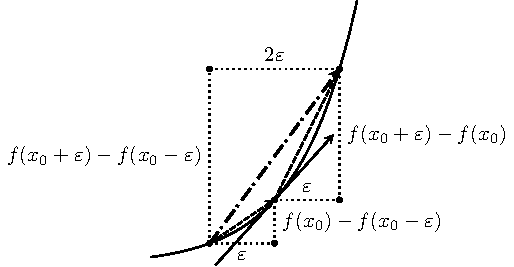
\includegraphics[width=.6\textwidth]{Chapters/04_GradientDescent/GD/latex/check_grad.pdf}
}
\end{figure}

Quan sát Hình~\ref{fig:explain_numgrad}, vector nét liền là đạo hàm {chính xác}
của hàm số tại điểm có hoành độ bằng $x_0$. Hai vector nét đứt thể hiện xấp xỉ
đạo hàm phía phải và phía trái. Vector chấm gạch thể hiện xấp xỉ đạo hàm hai
phía. Trong ba vector xấp xỉ đó, vector chấm gạch gần với vector nét liền nhất
nếu xét theo hướng.

Sự khác biệt giữa các phương pháp xấp xỉ còn lớn hơn nữa nếu tại điểm $x$, hàm số bị
{bẻ cong} mạnh hơn. Khi đó, xấp xỉ trái và phải sẽ khác nhau rất nhiều.
Xấp xỉ hai phía sẽ cho kết quả ổn định hơn.

% Từ đó ta thấy rằng xấp xỉ đạo hàm hai phía là xấp xỉ tốt hơn.

% \textbf{Với hàm nhiều biến}
\subsection{Xấp xỉ gradient của hàm nhiều biến}

Với hàm nhiều biến, công thức~\eqref{eqn:numgrdef2} được áp dụng cho từng biến
khi các biến khác cố định. Cụ thể, ta sử dụng định nghĩa gradient của hàm số nhận
đầu vào là một ma trận như công thức~\eqref{eqn:grmatrix1}. Mỗi thành phần của
ma trận kết quả là đạo hàm riêng của hàm số tại thành phần đó khi ta coi các thành
phần còn lại cố định. Chúng ta sẽ thấy rõ điều này hơn ở cách lập trình so sánh
hai cách tính gradient ngay sau đây.

Cách tính gradient xấp xỉ hai phía thường cho giá trị khá chính xác. Tuy nhiên,
cách này không được sử dụng để tính gradient vì độ phức tạp quá cao so với cách
tính trực tiếp. Tại mỗi thành phần, ta cần tính giá trị của hàm số tại phía trái
và phía phải. Việc làm này không khả thi với các ma trận lớn. Khi so sánh đạo
hàm xấp xỉ với gradient tính theo công thức, người ta thường giảm số chiều dữ
liệu và giảm số điểm dữ liệu để thuận tiện cho tính toán. Nếu gradient tính được
là chính xác, nó sẽ rất gần với gradient xấp xỉ này.

Đoạn code dưới đây giúp kiểm tra gradient của một hàm số khả vi $f:
\R^{m \times n} \rightarrow \R$, có kèm theo hai ví dụ. Để sử dụng hàm kiểm tra
\pythoninline{check_grad} này, ta cần viết hai hàm. Hàm thứ nhất là hàm
\pythoninline{fn(X)} tính giá trị của hàm số tại \pythoninline{X}. Hàm thứ hai
là hàm \pythoninline{gr(X)} tính giá trị của gradient của \pythoninline{fn(X)}.

\newpage

\begin{lstlisting}[language=Python]
from __future__ import print_function
import numpy as np

def check_grad(fn, gr, X):
    X_flat    = X.reshape(-1) # convert X to an 1d array, 1 for loop needed
    shape_X   = X.shape                # original shape of X
    num_grad  = np.zeros_like(X)       # numerical grad, shape = shape of X
    grad_flat = np.zeros_like(X_flat)  # 1d version of grad
    eps       = 1e-6      # a small number, 1e-10 -> 1e-6 is usually good
    numElems  = X_flat.shape[0] # number of elements in X
    # calculate numerical gradient
    for i in range(numElems):          # iterate over all elements of X
        Xp_flat      = X_flat.copy()
        Xn_flat      = X_flat.copy()
        Xp_flat[i]  += eps
        Xn_flat[i]  -= eps
        Xp           = Xp_flat.reshape(shape_X)
        Xn           = Xn_flat.reshape(shape_X)
        grad_flat[i] = (fn(Xp) - fn(Xn))/(2*eps)

    num_grad = grad_flat.reshape(shape_X)

    diff = np.linalg.norm(num_grad - gr(X))
    print('Difference between two methods should be small:', diff)

# ==== check if grad(trace(A*X)) == A^T ====
m, n = 10, 20
A = np.random.rand(m, n)
X = np.random.rand(n, m)

def fn1(X):
    return np.trace(A.dot(X))

def gr1(X):
    return A.T

check_grad(fn1, gr1, X)
# ==== check if grad(x^T*A*x) == (A + A^T)*x  ====
A = np.random.rand(m, m)
x = np.random.rand(m, 1)

def fn2(x):
    return x.T.dot(A).dot(x)

def gr2(x):
    return (A + A.T).dot(x)

check_grad(fn2, gr2, x)

\end{lstlisting}
% \newpage
\kq
\begin{lstlisting}
Difference between two methods should be small: 2.02303323394e-08
Difference between two methods should be small: 2.10853872281e-09
\end{lstlisting}

Kết quả cho thấy sự khác nhau giữa Frobenious norm (norm mặc định trong
\pythoninline{np.linalg.norm}) trong kết quả của hai cách tính là rất nhỏ. Sau
khi chạy lại đoạn code với các giá trị \pythoninline{m, n} khác nhau và biến
\pythoninline{X} khác nhau, nếu sự khác nhau vẫn là nhỏ, ta có thể kết luận rằng
gradient mà ta tính được là chính xác.

Bạn đọc có thể kiểm tra lại các công thức trong Bảng~\ref{tab:commongr} bằng
phương pháp này.



